% !TeX root = ../main.tex
% !Mode:: "TeX:UTF-8"
\section{第八章 团队介绍}\label{ux7b2cux516bux7ae0-ux56e2ux961fux4ecbux7ecd}

PI OS 项目团队由软件工程、网络安全、人工智能及计算机科学与技术等专业的本科生、硕士生和博士生组成。团队围绕华为``高密部署智能体沙箱引擎''命题，将底层系统研究、工程验证与企业应用需求结合，推进技术实现、实验复核、商业测算和成果转化。

团队成员根据研究与工程经验承担系统研发、智能体机制说明、测试验证、安全分析、财务测算、文档规范和项目统筹等工作，并通过统一术语、数据复核与版本管理保持跨模块协作。

\subsection{8.1 主创团队}\label{ux4e3bux521bux56e2ux961f}

\subsubsection{8.1.1 团队构成与能力互补}\label{ux56e2ux961fux6784ux6210ux4e0eux80fdux529bux4e92ux8865}

项目以运行时扁平化、动态资源卸载和智能内存共享为核心技术方向，目前已完成现阶段核心代码开发。后续重点包括命题指定环境适配、性能与隔离测试、交付文档完善，以及在权属和授权边界明确后推进客户验证。

团队能力可归纳为系统基础设施、智能体运行优化、测试验证体系与产业转化体系四类，研究侧依托天津大学科研平台，产业侧依托与华为的技术合作，形成技术研发、企业需求、学生成长和成果转化相互衔接的协作结构。

\begin{longtable}[]{@{}
  >{\centering\arraybackslash}p{(\linewidth - 4\tabcolsep) * \real{0.1406}}
  >{\centering\arraybackslash}p{(\linewidth - 4\tabcolsep) * \real{0.3038}}
  >{\raggedright\arraybackslash}p{(\linewidth - 4\tabcolsep) * \real{0.5556}}@{}}
\caption*{表 8-1 PI OS 项目成员与现阶段分工}\tabularnewline
\toprule\noalign{}
\rowcolor{WordTableHeader}
\begin{minipage}[b]{\linewidth}\centering
\TableHeaderText{姓名}
\end{minipage} & \begin{minipage}[b]{\linewidth}\centering
\TableHeaderText{年级与专业}
\end{minipage} & \begin{minipage}[b]{\linewidth}\centering
\TableHeaderText{现阶段职责}
\end{minipage} \\
\midrule\noalign{}
\endfirsthead
\toprule\noalign{}
\rowcolor{WordTableHeader}
\begin{minipage}[b]{\linewidth}\centering
\TableHeaderText{姓名}
\end{minipage} & \begin{minipage}[b]{\linewidth}\centering
\TableHeaderText{年级与专业}
\end{minipage} & \begin{minipage}[b]{\linewidth}\centering
\TableHeaderText{现阶段职责}
\end{minipage} \\
\midrule\noalign{}
\endhead
\bottomrule\noalign{}
\endlastfoot
\rowcolors{1}{WordTableStripe}{white}
张纪同 & 2023 级本科 · 软件工程 & 项目统筹、命题需求对齐、计划书整合与答辩组织 \\
陈奕池 & 2026 级博士 · 软件工程 & 核心代码实现、运行时机制研发与技术评审支持 \\
刘国威 & 2024 级博士 · 计算机科学与技术 & 性能优化与技术路线可行性论证支持 \\
周以恒 & 2026 级硕士 · 计算机科学与技术 & 系统研究、技术文档审核与方案复核支持 \\
范文丽 & 2024 级本科 · 软件工程 & 财务分析与融资计划、团队材料整理与协作证据 \\
李子鹏 & 2025 级本科 · 计算机科学与技术 & 测试数据复核、指标计算、测试环境与验收材料 \\
刘书雄 & 2024 级本科 · 人工智能 & 智能体任务流程、动态卸载与预取机制说明 \\
王子硕 & 2025 级本科 · 网络安全 & 隔离与共享安全、数据保护及风险管理材料 \\
王新雅 & 2025 级本科 · 软件工程 & 文档规范、来源整理、术语统一与复现说明 \\
张思淼 & 2025 级本科 · 软件工程 & 运行时扁平化方案、组件职责与架构说明 \\
\end{longtable}

\begin{quote}
注：表中职责对应当前项目推进阶段，具体贡献通过代码、测试数据、文档版本和协作记录等材料留存。
\end{quote}

\begin{center}
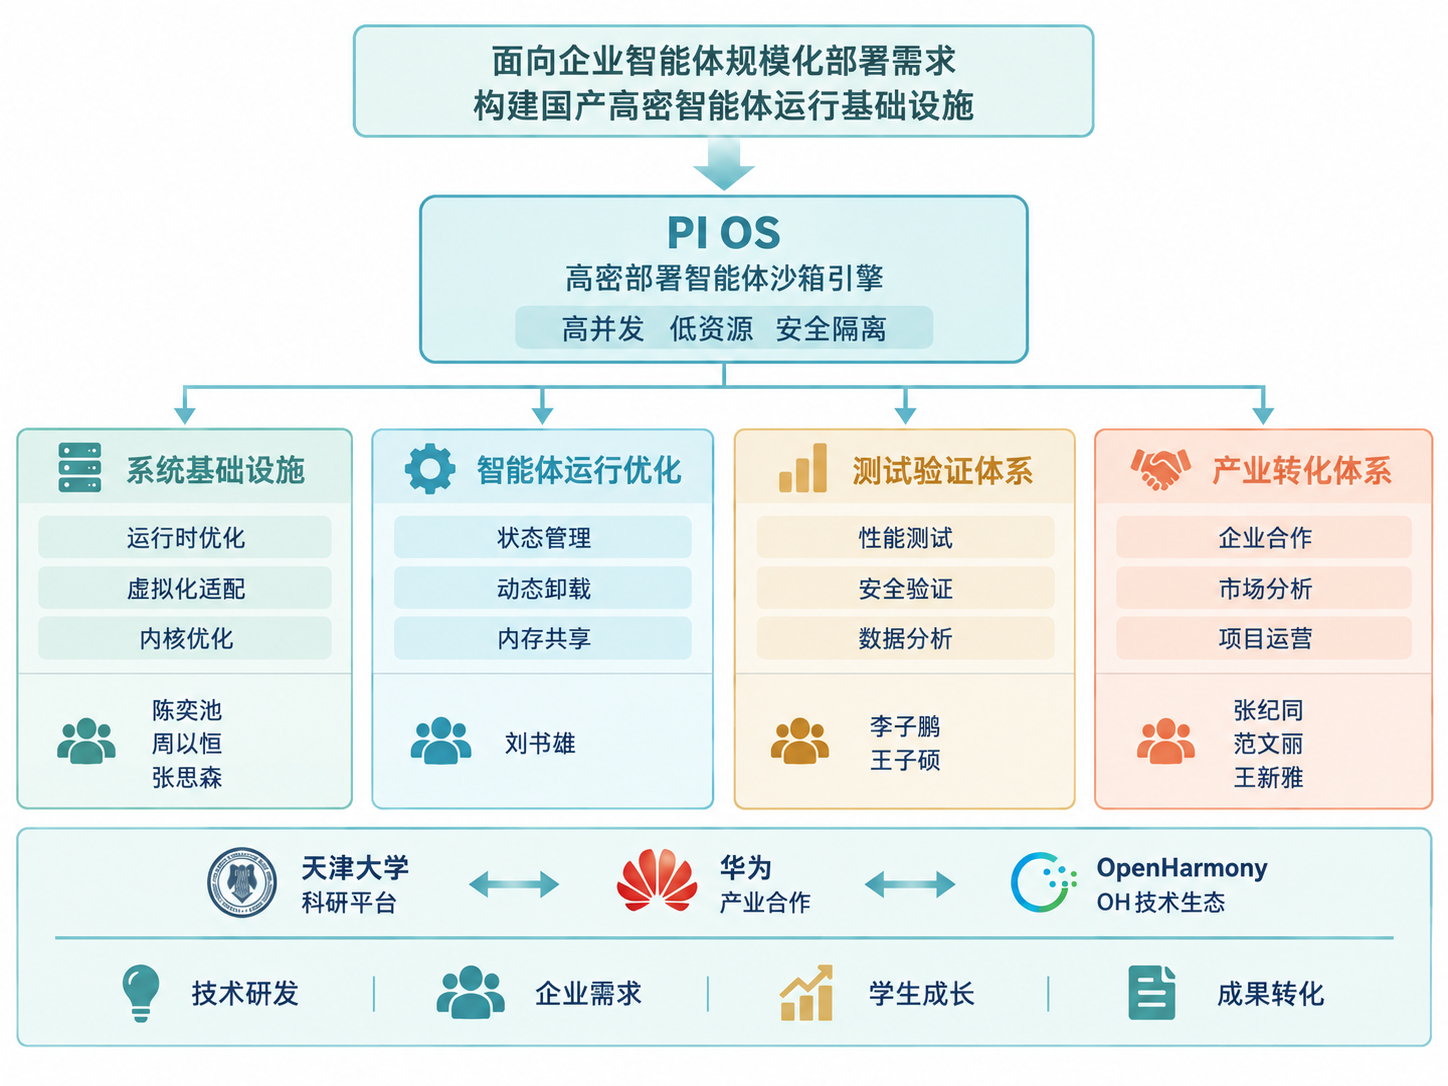
\includegraphics[width=5.6in,keepaspectratio]{figures/image26.png}
\end{center}
\WordFigureCaption{图 8-1 PI OS 高密部署智能体沙箱引擎项目组织与研发体系}

\subsubsection{8.1.2 协作与质量控制机制}\label{ux534fux4f5cux4e0eux8d28ux91cfux63a7ux5236ux673aux5236}

项目采用模块责任制和交叉复核机制。每项核心内容明确主责人、输入材料、结论和复核方式，技术指标保留原始数据、脚本与环境说明，经营数字保留计算依据与关键假设。

\begin{longtable}[]{@{}
  >{\centering\arraybackslash}p{(\linewidth - 4\tabcolsep) * \real{0.1953}}
  >{\raggedright\arraybackslash}p{(\linewidth - 4\tabcolsep) * \real{0.6172}}
  >{\raggedright\arraybackslash}p{(\linewidth - 4\tabcolsep) * \real{0.1875}}@{}}
\caption*{表 8-2 团队协作与质量控制机制}\tabularnewline
\toprule\noalign{}
\rowcolor{WordTableHeader}
\begin{minipage}[b]{\linewidth}\centering
\TableHeaderText{机制}
\end{minipage} & \begin{minipage}[b]{\linewidth}\centering
\TableHeaderText{执行方式}
\end{minipage} & \begin{minipage}[b]{\linewidth}\centering
\TableHeaderText{作用}
\end{minipage} \\
\midrule\noalign{}
\endfirsthead
\toprule\noalign{}
\rowcolor{WordTableHeader}
\begin{minipage}[b]{\linewidth}\centering
\TableHeaderText{机制}
\end{minipage} & \begin{minipage}[b]{\linewidth}\centering
\TableHeaderText{执行方式}
\end{minipage} & \begin{minipage}[b]{\linewidth}\centering
\TableHeaderText{作用}
\end{minipage} \\
\midrule\noalign{}
\endhead
\bottomrule\noalign{}
\endlastfoot
\rowcolors{1}{WordTableStripe}{white}
页面/模块责任制 & 每项核心内容明确主责人、输入材料、结论与复核人 & 明确责任边界 \\
证据留存 & 技术指标保留原始数据、脚本、环境说明和复现步骤；经营数字保留计算依据 & 保证材料可复核 \\
交叉复核 & 技术页由非主责成员检查逻辑和可读性，关键数据至少完成一次独立复算 & 降低单点错误 \\
统一口径 & 项目名称、技术状态、指标口径、商业化边界在计划书、PPT 和答辩中保持一致 & 提高交付一致性 \\
版本与交接 & 保留代码、测试报告、计划书和展示材料版本；关键模块同步整理部署方法和待办 & 保障项目连续性 \\
\end{longtable}

底层系统开发、工程测试、财务测算和商业表达相互校验：技术结果决定可对外说明的产品能力，测试数据支撑性能与价值判断，财务测算则反向约束人员扩张和客户定价，使技术、市场和财务保持同一套项目口径。

\subsubsection{8.1.3 学生成长与项目持续性}\label{ux5b66ux751fux6210ux957fux4e0eux9879ux76eeux6301ux7eedux6027}

团队把企业真实需求转化为可执行的学生实践任务。新成员从环境搭建、测试复现、文档完善和小范围问题修复开始参与，关键修改经评审后合入；个人贡献以任务成果、复核质量和协作记录共同体现。

随着项目进入商业化阶段，团队将根据真实订单和交付负荷补充产品、运维及商务能力。新增岗位以实际工作瓶颈为依据，并通过技术文档、权限交接和备份负责人机制降低人员变化对项目连续性的影响。

\subsection{8.2 指导教师}\label{ux6307ux5bfcux6559ux5e08}

本项目指导教师为天津大学赵来平教授。赵来平教授研究领域为计算系统，研究方向包括数据中心、云计算、软件定义网络和智能运维，主讲云计算课程并承担研究生指导工作，其研究方向与 PI OS 涉及的智能体运行环境、计算资源管理和系统运行效率优化具有较高相关性。

项目推进过程中，指导教师主要负责技术路线、实验方法和关键问题把关，具体的方案分析、代码实现、实验复核、财务测算和材料整理由团队成员按分工完成。该协作方式既保证技术方向和实验方法的规范性，也保留学生团队在项目实现与交付中的主体作用。

